% samplepaper.tex: springer.com
% modificato da MM 06/05/2018
%
\documentclass[runningheads]{llncs}
\usepackage[italian]{babel}
\usepackage{graphicx}
\usepackage{subfigure}
\usepackage{listings}
\usepackage{threeparttable}
% Used for displaying a sample figure. If possible, figure files
% should be included in EPS format.  If you use the hyperref package,
% please uncomment the following line to display URLs in blue roman
% font according to Springer's eBook style:
% \renewcommand\UrlFont{\color{blue}\rmfamily}
\begin{document}
%
\title{Sistema IR per collezione di articoli medici uilizzando diversi insiemi di stopword}
%
% \titlerunning{Abbreviated paper title}
% If the paper title is too long for the running head, you can set
% an abbreviated paper title here
%
\author{%
  Alessandro Stefani\inst{1} \and
  Caterina Buranelli\inst{2} \and
  Cristi Gutu\inst{3}}
%
\authorrunning{Alessandro Stefani, Caterina Buranelli, Cristi Gutu}
% First names are abbreviated in the running head.  If there are more
% than two authors, 'et al.' is used.
%
\institute{Corso di laurea in Statistica per le tecnologie e le scienze,
  matricola 1148387 \email{alessandro.stefani.6@studenti.unipd.it} \and Corso di laurea in Statistica per le tecnologie e le scienze,
    matricola 1234567 \email{caterina.buranelli@studenti.unipd.it} \and Corso di laurea in Statistica per le tecnologie e le scienze,
      matricola 1147351 \email{gheorghecristi.gutu@studenti.unipd.it}
  }
%
\maketitle
% typeset the header of the contribution
%
\begin{abstract}
DA FINIRE QUANDO ABBIAMO MESSO A POSTO LA SEZIONE ESPERIMENTI.
Questo progetto tratta la realizzazione attraverso il pacchetto \emph{Whoosh}, di un motore di ricerca
volto al reperimento di documenti della collezione sperimentale \emph{OHSUMED} indicizzata opportunamente.
Il progetto è anche corredato di un webserver che permette all'utente di interrogare il motore di ricerca
in forma interattiva attraverso un browser a scelta.
 \keywords{{\it
      Information Retrieval  \and IR \and statistica \and reperimento \and indicizzazione \and Whoosh \and Python \and webserver \and web \and interrogazione web}}
\end{abstract}

\section{Introduzione}
\label{sec:introduzione}

Lo scopo finale di un Sistema di Information Retrieval (IRS) \`e quello di reperire documenti
 rilevanti relativi a una certa esigenza informativa\footnote{insieme delle circostanze in cui una
 persona ha un problema da risolvere o un compito da svolgeree richiede informazioni
 importanti, utili o necessarie per la risoluzione del problema o lo svolgimento del compito};
  dunque i documenti sono il primo input del sistema, mentre il secondo \`e
  costitutito dalle interrogazioni; i documenti devono essere
  indicizzati e nell'indice creato, si andr\`a a effettuare la ricerca per reperire documenti rilevanti\footnote{la rilevanza e' la proprieta' che rende l'informazione importante, utile o necessaria a soddisfare l'esigenza informativa dell'utente}. Questa seconda parte e' detta reperimento e non si occupa solo di ricercare tra i documenti, ma anche di riordinare secondo un certo ordine di rilevanza. Cio' che descrive i documenti e cio' che descrive le interrogazioni deve essere confrontabile, infatti nei programmi di indicizzaizone e di reperimento si usa uno schema, che deve essere uguale
  in entrambi i casi.
L'indicizzazione \`e un trade-off tra il  miglioramento della rapprerentazione del
contenuto informativo dei documenti (efficacia) e la gestione degli indici (efficienza).
Esistono diversi modi per risolvere questo problema, nel nostro caso abbiamo ricercato
la configurazione migliore tra un sistema di reperimento con o senza uso di stopword.


Il resto della relazione \`e organizzato come segue. Nella sezione 2, si descrivono
alcuni dei metodi standard, i pi\`u didattici, su cui si basano gli esperimenti.
La sezione 3, presenta l'interfaccia web e le sue modalit\`a di utilizzo.
Nella sezione 4, sono riportati gli esperimenti fatti ed i risultati ottenuti,
commentati e sotto forma di tabelle esplicative. Infine, nella sezione 5,
si traggono delle brevi conclusioni.




L'obiettivo principale della relazione \`e da una parte la
documentazione del progetto di un servizio di {IR} e dall'altra una
misura del grado in cui si sia riusciti a mettere in pratica i
contenuti della disciplina illustrati durante le lezioni.

A tal scopo la relazione dovr\`a illustrare nelle sezioni successive:
\begin{itemize}
\item i metodi di indicizzazione,
\item i modelli di reperimento,
\item l'interfaccia basata su un \textit{browser} per il {WWW}
\item i risultati della \emph{valutazione} condotta con la collezione
  sperimentale OHSUMED.
\end{itemize}
Il lettore della relazione \`e lo studente medio di un corso di laurea
in statistica al quale la relazione deve dare tutti gli strumenti per
comprendere il contenuto.  Ci si metta nei suoi panni e si scriva
tutto ci\`o e solo ci\`e che serve.  Chiedersi qual \`e il messaggio
che lo studente deve ``portarsi a casa'', esplicitarlo in questo
paragrafo e concentrarsi su quello nel resto della relazione.

L'introduzione della relazione deve servire al lettore a capire se
vale la pena continuare a leggere il resto.  Si possono riassumere i
contenuti delle sezioni successive e metterne in evidenza i punti
principali.  La relazione consiste di tre paragrafi principali dopo
questa introduzione e prima della bibliografia, per la quale si
suggerisce Bib\TeX\ se si scrive con \LaTeX.

\section{Base di partenza}
\label{sec:base-di-partenza}

Un metodo utilizzato per tutti gli esperimenti \`e il cos\`i detto
"Best Match 25 Model with Extension to Multiple Weighted Fields" o in breve BM25F


Le stopword\cite{WBC_stopword} sono parole che non portano informazione
significativa al contenuto informativo come congiunzioni, articoli, avverbi..\par

%
%\section{Metodi proposti}
%\label{sec:metodi-utilizzati}
%
%Nel caso in cui si siano sviluppati:
%\begin{itemize}
%\item modelli di reperimento,
%\item metodi di indicizzazione,
%\item schemi di pesatura o
%\item altri metodi o tecniche
%\end{itemize}
%propri, non documentati in libri di testo o altra letteratura, si
%scriva in questa sezione una descrizione accurata e completa.  Si
%mettano in evidenza le caratteristiche distintive dei propri
%contributi.  Se non si \`e proposto nulla di nuovo, si scriva
%\emph{Nessuno}.  In una delle ultime lezioni si vedr\`a come
%implementare delle proprie funzioni di reperimento e schemi di
%pesatura.


\section{Interfaccia web}


\section{Esperimenti e Risultati}
\label{sec:esperimenti}


Per gli esperimenti si \`e utilizzata parte della gi\`a citata collezione sperimentale chiamata OHSUMED\footnote{ \url{https://bit.ly/2wpOynZ}}.

Si tratta di una collezione di oltre 300'000 articoli provenienti dal database bibliografico MEDLINE pubblicati tra il 1987 ed il 1991, di questi documenti ne sono stati utilizzati 54'711.

I programmi utilizzati per effettuare indicizzazione e reperimento sono stati scritti in python(versione 2.7), sfruttando oggetti e funzioni del modulo whoosh\footnote{ \url{https://whoosh.readthedocs.io/en/latest/index.html}}.

Per la valutazione dei risultati ottenuti nei vari esperimenti si \`e invece utilizzato lo strumento standard trec\_eval\footnote{ \url{https://trec.nist.gov/trec\_eval/}}.
Questo programma permette di ottenere alcune misure della qualit\`a di un sistema di information retrieval se si conoscono i documenti rilevanti per le query sperimentali utilizzate.

Come misura da usare nel confronto tra risultati di diverse run si \`e scelta la Mean Average Precision(MAP)\cite{WBC_map} , quantit\`a calcolabile sia a livello di singola query che a livello complessivo su un insieme di query.
Inoltre, per verificare se i valori di MAP ottenuti in run diverse si discostano in modo statisticamente significativo gli uni dagli altri si effettuano test di Wilcoxon\cite{} su coppie di risultati. \par

\subsection{Scelte iniziali}

Prima di iniziare gli esperimenti sono state fatte delle scelte riguardo certi aspetti dei metodi di reperimento che rimanessero costanti durante tutti gli esperimenti.
Queste scelte sono state fatte in seguito ad alcune run preliminari.

Per la funzione di reperimento e ranking come schema di pesatura si \`e deciso di utilizzare il BM25F, descritto nella sezione precedente, inquanto "state-of-the-art" dal punto di vista dei modelli per information retrieval su documenti strutturati, e come operatore logico per raggruppare le parole delle query si \`e deciso di utilizzare l'operatore OR, ovvero si cercano documenti in cui \`e presente almeno una parola della query.

Sempre a seguito delle run preliminari si \`e deciso di utilizzare il campo "desc" delle query anzich\`e il campo "title" inquanto d\`a risultati migliori, inoltre, si \`e notato che in alcune query sperimentali sono presenti parole scritte in modo errato e che quindi non risultano presenti nell'indice.
Per questo dopo aver verificato, leggendo i documenti rilevanti per quelle query, quali fossero gli errori si \`e ritenuto opportuno effettuare una correzione al momento del reperimento.
A grandi linee, la correzione viene fatta su parole che non risultano presenti nell'indice cercando in quest'ultimo delle parole alternative che si discostano di al pi\`u una lettera dalla parola originale; queste parole vengono quindi aggiunte alla query di partenza e si procede con la ricerca.

Un'ultima scelta \`e stata fatta riguardo il numero massimo di documenti reperiti.
Si \`e optato per 100 documenti poiche un numero maggiore non porta grandi miglioramenti dal punto di vista del MAP. \par

\vskip 1in
Affinch\`e Whoosh possa indicizzare una collezione di documenti, necessita la
specificazione di uno schema che include, per ogni possibile campo dei documenti della collezine, il nome del campo ed il tipo del campo.

Lo schema di base per la collezione qui utilizzata \`e il seguente:
\par

\begin{figure}
\begin{lstlisting}
schema = Schema(docid      	= ID(stored=True),
		title      	= TEXT(stored=True),
		identifier	= ID(stored=True),
		terms 		= NGRAM(stored=True),
		authors		= NGRAM(stored=True),
		abstract 	= TEXT(stored=True),
		publication	= TEXT(stored=True),
		source 		= TEXT(stored=True))
\end{lstlisting}
      \caption{Schema necessario all'indicizzazione dei documenti. "stored=True" indica che il campo viene salvato ed \`e quindi successivamente accessibile. }
\end{figure}



%\vskip 1in

\subsection{Baseline}
I valori di MAP scelti come baseline sono quelli ottenuti effettuando ricerche su un indice con lo schema di base, riportato sopra, senza l'utilizzo di una lista di stopword e cercando in due campi dei documenti: "title" e "abstract".
Cercando su un campo ("title") o tre campi ("title", "abstract" e "terms") risulta solo in un peggioramento dei risultati.

Si possono vedere i risultati ottenuti usando la configurazione "baseline" riassunti in Tabella 1.
\par


\begin{table}
\centering
\begin{tabular}{lll}
\hline
\textbf{ un campo }           & \textbf{ due campi }           & \textbf{ tre campi }            \\ \hline
 num\textit{q all 63 }       &  num\textit{q all 63 }       &  num\textit{q all 63 }        \\
 num\textit{ret all 6228 }  &  num\textit{ret all 6244 }  &  num\textit{ret all 6271 }   \\
 num\textit{rel all 670 }    &  num\textit{rel all 670 }    &  num\textit{rel all 670 }     \\
 num\textit{rel}ret all 349  &  num\textit{rel}ret all 419  &  num\textit{rel}ret all 367   \\
map all 0.2130               & map all \bf 0.2744               & map all 0.2155 \\ \hline
\end{tabular}

\caption{ Risultati treceval complessivi per tutte le query, nessuna manipolazione del testo, numero risultati restituiti per
ogni query = 100, pesatura BM25F.}
\end{table}

Come si nota dalla tabella il valore baseline di \textit{M.A.P} \`e 0.2744.
\par

%
%  Il processo ed il codice per creare l'indice sono  facilmente comprensibili visionando il file  \emph{indicizzatore\_batch\_baseline.py}. \par
% \lstset{
%   language=bash,
%   basicstyle=\ttfamily
% }
%
% Per eseguire l'indicizzazione  baseline \`e sufficiente lanciare lo script python con il seguente comando:
% \begin{lstlisting}
%   indicizzatore_batch_baseline.py \
%   cartella_indice file_documenti.xml
% \end{lstlisting}
%
% Per eseguire il reperimento, che poi produce il file con i risultati in formato compatibile con trec\_eval, \`e sufficiente lanciare lo script python con il comando:
%
% \begin{lstlisting}
%   python search_tk.py cartella_indice \
%   file_query.xml cartella_risultati nome_file_risultati
% \end{lstlisting}





\subsection{Esperimenti}

Gli esperimenti sono consistiti in tre prove in cui si cambia l'insieme di stopword usato nell'indicizzazione. In particolare ad ogni prova si utilizza un insieme di stopword con parole in pi\`u rispetto a quello delle prove precedenti.

Come con la baseline, per ciascuna prova si effettua la ricerca per uno, due e tre campi.

\subsubsection{Prima prova:}

Per la prima prova sono state utilizzate le stopword generali della lingua inglese. Queste comprendono termini come "the", "that", "is"; sono poi state aggiunte anche le lettere dell'alfabeto ed i numeri.

Come si vede in Tabella 2, non sembra si sia ottenuto un miglioramento significativo rispetto alla baseline. Il MAP ottenuto utilizzando due campi "migliora" solo dello 0.0001.
\begin{table}
\centering
\begin{tabular}{lll}
\hline
\textbf{ un campo }           & \textbf{ due campi }           & \textbf{ tre campi }            \\ \hline
 num\textit{q all 63 }       &  num\textit{q all 63 }       &  num\textit{q all 63 }        \\
 num\textit{ret all 6228 }  &  num\textit{ret all 6244 }  &  num\textit{ret all 6271 }   \\
 num\textit{rel all 670 }    &  num\textit{rel all 670 }    &  num\textit{rel all 670 }     \\
 num\textit{rel}ret all 350  &  num\textit{rel}ret all 418  &  num\textit{rel}ret all 367   \\
map all 0.2137               & map all \bf 0.2745               & map all 0.2152          \\ \hline
\end{tabular}

\caption{ Risultati treceval, rimozione delle stopword generali, numero risultati restituiti per ogni query = 100, pesatura BM25F.}
\end{table}

\subsubsection{Seconda prova:}

Nella seconda prova si \`e allora cercato di migliorare i risultati aggiungendo alle stopword generali, alcune parole che non sono normalmente considerate stopword ma che nel contesto medico, come nel caso della collezione OHSUMED, diventano tali.

Per questo abbiamo utilizzato un insieme di stopword denominate stopword\_cliniche che oltre ad avere le stopword generali ha anche parole come "medical", "condition" o "family"\footnote{ \url{https://github.com/kavgan/clinical-concepts/blob/master/clinical-stopwords.txt}}.

Con questa prova sono stati ottenuti risultati accettabili, infatti come si vede in Tabella 3, l'aumento del MAP rispetto alla baseline \`e stato quasi dello 0.01:
\begin{table}
\centering
\begin{tabular}{lll}
\hline
\textbf{ un campo }           & \textbf{ due campi }           & \textbf{ tre campi }            \\ \hline
 num\textit{q all 63 }       &  num\textit{q all 63 }       &  num\textit{q all 63 }        \\
 num\textit{ret all 6228 }  &  num\textit{ret all 6244 }  &  num\textit{ret all 6271 }   \\
 num\textit{rel all 670 }    &  num\textit{rel all 670 }    &  num\textit{rel all 670 }     \\
 num\textit{rel}ret all 350  &  num\textit{rel}ret all 419  &  num\textit{rel}ret all 376   \\
map all 0.2156               & map all \bf 0.2837               & map all 0.2166          \\ \hline
\end{tabular}

\caption{ Risultati treceval, rimozione delle stopword cliniche, numero risultati restituiti per ogni query = 100, pesatura BM25F.}
\end{table}


\subsubsection{Terza prova:}

Nell'ultima prova sono state aggiunte altre parole alla lista delle stopword. La scelta delle parole da aggiungere \`e stata fatta in due fasi principali.

Nella prima \`e stata ricavata la frequenza con cui le parole delle query appaiono nei rispettivi documenti rilevanti. Dopo di ci\`o le parole con frequenza prossima allo 0 sono state prese in considerazione come possibili stopword.

Nella seconda fase sono state prese le query che, basandosi sui risultati della seconda prova, hanno avuto un MAP relativamente basso(inferiore a 0.2). Sono state quindi prese alcune parolo di queste query come altre possibili stopword anche basandosi sulla loro frequenza nei documenti rilevanti.

Per alcune parole la scelta se includerle nell'insieme di stopword \`e stata resa difficile dal fatto che, essendo presenti in pi\`u di una query la loro rimozione poteva significare il miglioramento di un MAP ed il peggioramento di un altro.

Per questo, prima di arrivare all'insieme finale sono stati fatti alcuni tentativi.

%prima prendendo in considerazione le parole delle query e la frequenza con cui queste si trovano nei documenti rilevanti e poi cercando la presenza di possibili stopword nelle query che davano risultati peggiori.



Come si pu\`o notare dalla Tabella 4 si ha un aumento del MAP rispetto alla baseline decisamente superiore alle prove precedenti, con circa lo 0.075 in pi\`u.
\begin{table}
\centering
\begin{tabular}{lll}
\hline
\textbf{ un campo }           & \textbf{ due campi }           & \textbf{ tre campi }            \\ \hline
 num\textit{q all 63 }       &  num\textit{q all 63 }       &  num\textit{q all 63 }        \\
 num\textit{ret all 5282 }  &  num\textit{ret all 5690 }  &  num\textit{ret all 5788 }   \\
 num\textit{rel all 670 }    &  num\textit{rel all 670 }    &  num\textit{rel all 670 }     \\
 num\textit{rel}ret all 386  &  num\textit{rel}ret all 463  &  num\textit{rel}ret all 435   \\
map all 0.2720               & map all \bf 0.3508               & map all 0.2813          \\ \hline
\end{tabular}

\caption{ Risultati treceval, rimozione delle stopword cliniche migliorate, numero risultati restituiti per ogni query = 100, pesatura BM25F.}
\end{table}
\par

La Figura 2 riassume i risultati delle tre prove e si pu\`o notare un netto miglioramento utilizzando le stopword migliorate.


\begin{figure}%
    \centering
    {{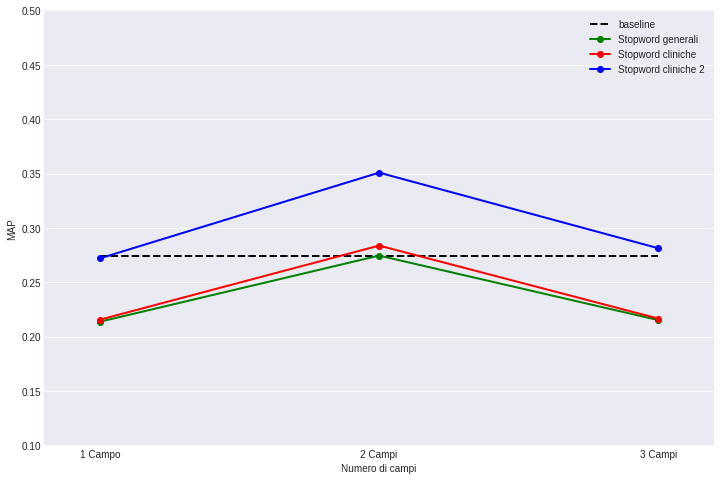
\includegraphics[width=1\linewidth]{maps} }}%
    \caption{Variazione del MAP campbiando il numero di campi per i tre insiemi di stopword, la linea orizzontale indica la baseline di 0.2744.}%
\end{figure}


\subsection{Test di significativit\`a :}
Per avere conferma che le differenze tra i MAP ottenuti nelle varie prove e nella baseline
siano significativamente diversi si \`e ritenuto opportuno effettuare dei test.
Tra i test che si utilizzano comunemente a questo scopo si \`e scelto di utilizzare il
test di Wilcoxon che a differenza dell'alternativo t-test risulta avere pi\`u
potenza statistica in caso di non normalit\`a dei dati.

I test sono stati fatti tra i MAP delle prove utilizzando due campi in quanto hanno
dato generalmente risultati migliori.

L'ipotesi alternativa \`e unilaterale ed equivale a dire che, tra le due prove
confrontate, la seconda prova ha MAP maggiore della prima.
Per contro l'ipotesi nulla \`e che la prima prova ha MAP maggiore o uguale alla seconda.

\begin{table}
\centering
\begin{tabular}{lll}
\hline
\textbf{ Prove a confronto }  & \textbf{ statistica test }  & \textbf{ p-value }            \\ \hline
 BASELINE contro STOP1  &  582      &  0.0393       \\
 BASELINE contro STOP2  &  551.5    &  0.0092       \\
 STOP1 contro STOP2     &  549.5    &  0.0056       \\
 BASELINE contro STOP3  &  276.0    &  $1.2749\mathrm{e}{-6}$   \\
 STOP1 contro STOP3     &  291.0    &  $1.2936\mathrm{e}{-6}$   \\
 STOP2 contro STOP3     &  290.0    &  $3.5437\mathrm{e}{-6}$   \\ \hline
\end{tabular}

\caption{ Statistiche test e livelli di significativit\`a osservati per i test sulla differenza dei MAP.
STOP1 indica le stopword generali, STOP2 indica le stopword cliniche e STOP3 indica le stopword cliniche migliorate.}
\end{table}

Come si vede in Tabella 5 i miglioramenti portati dalle stopword delle prime due prove hanno p-value che permettono di rifiutare l'ipotesi nulla solo in caso si prenda come soglia il livello di significativit\`a dello 0.05.
Invece, con la terza prova il p-value risulta molto pi\`u basso portando a rifiutare l'ipotesi nulla in maniera pi\`u convincente.


\section{Conclusione}

Come si \`e visto dai risultati delle prove, l'utilizzo di stopword inerenti al contesto
della collezione, porta a reperire pi\`u documenti rilevanti nelle prime posizioni.
Bisogna, per\`o, tenere in considerazione che nella terza prova, quella che ha dato
i risultati migliori, l'insieme delle stopword creato \`e strettamente legato alle
query sperimentali. Per questo c'\`e la possibilit\`a che i risultati ottenuti con query diverse
siano peggiori.


%
%Inizialmente si \`e pensato che utilizzare le stopword generali della lingua inglese fosse sufficiente per eliminare le
%parole che non portano informazione, e di conseguenza aumentare il parametro di interesse M.A.P; i risultati
%non sono stati molto soddisfacenti, abbiamo quindi optato per l'utilizzo di stopword cliniche, cio\`e stopword utilizzate
%soltato in ambito clinico/medico \cite{stopword_cliniche}.

\begin{thebibliography}{8}

\bibitem{WBC}
W. Bruce Croft and Donald Metzler and Trevor Strohman. Search Engines: Information Retrieval in Practice. Addison Wesley, (2009), pp. 250-252

\bibitem{WBC_stopword}
W. Bruce Croft and Donald Metzler and Trevor Strohman. Search Engines: Information Retrieval in Practice. Addison Wesley, (2009), pp. 90

\bibitem{WBC_map}
W. Bruce Croft and Donald Metzler and Trevor Strohman. Search Engines: Information Retrieval in Practice. Addison Wesley, (2009), pp. 313

\end{thebibliography}

\begin{figure}[h!]
  \subfigure[Alessandro Stefani]{
    
\includegraphics[width=35mm,height=35mm]{aleste}}
  \subfigure[Caterina Buranelli]{
    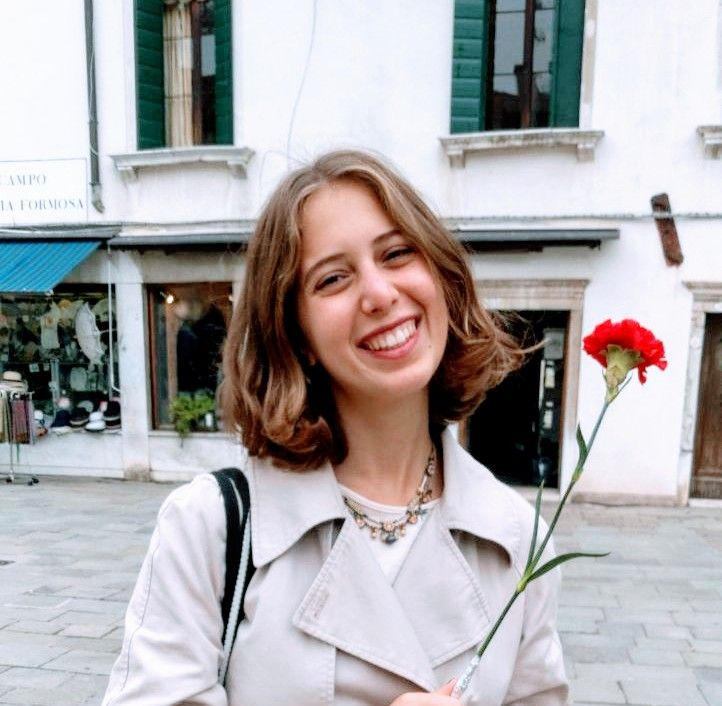
\includegraphics[width=35mm,height=35mm]{caterina}}
  \subfigure[Cristi Gutu]{
    
\includegraphics[width=35mm,height=35mm]{cristi}}
\end{figure}

\end{document}
